\chapter{Modelling a bio-inspired series-viscoelastic actuator} \label{ch7:ModelingBio}

\section{Introduction}

In the previous chapters, two modelling tools for the prediction of the viscoelastic behaviour of soft materials were developed. Their prediction capabilities were assessed, being the ANN model more accurate in accounting for the velocity-dependent stress response of the soft materials. Nonetheless, a further validation must be performed to corroborate current findings. 

The motivation behind developing modelling tools to account for the viscoelastic behaviour of soft materials, is to deploy this tool into real robotic applications. Therefore, this chapter presents a preliminary concept design of a bio-inspired series-viscoelastic actuator. The experimental validation is aimed to be done in future works. Nonetheless, many information regarding the design process of the latter actuator was compiled and is presented in here.

Moreover, the performance of the ANN model in real-time is assessed by exporting the developed ANN model to Simulink. The stress response of the model is observed for several different input signals. Results highlight an unexpected limitation of the developed ANN model which is not able to perform well under a variable strain rate input. This can be circumvented by keeping the strain rate input constant. However, this is a limitation which must be addressed for the ANN model to be reliable in real robotics applications.

In summary, the design process presented in here consists of: the selection of the best soft material to match the human tendon properties; the selection of the electric motor and gearbox combination suitable to deliver 50\% assistance, based on the knee torque requirements during walking activities; the evaluation of the ANN model in real time under different strain input signals; the experimental protocol proposed, based on mimicking the human muscle skeletal system functionality, and the 3D design of a clamping device aimed to hold several pieces of soft materials in a bundle-form.

\section{Matching the Human Tendon Properties}

In line with the aim of implementing the human skeletal muscle system functionality in soft robotic applications, i.e. a bio-inspired soft actuator, this section presents a comparison analysis between the mechanical properties of the seven studied soft materials, and the human tendons and ligaments involved in the motion of the knee joint. The latter is motivated due to the large participation this joint has on the activities of daily living (\Cref{sec:mimicHSMS}.) 

Moreover, it is desired to identify which of the studied soft materials is able to match the human tendon mechanical properties. Therefore, the first step of this process is to extract the viscoelastic properties of the patellar tendon and the quadriceps ligament \cite{schatzmann1998effect,staubli1999mechanical,johnson1994tensile}. Subsequently, the extracted data is compiled into the following table for direct comparison

\begin{table}[htbp!]
    \centering
    \caption{Viscoelastic properties of the quadriceps tendon compared against the studied soft materials. The ultimate strength values are from the 50 mm/min test. The full parameters list can be found in \Cref{tbl:stressRelProperties,tbl:elasticProp}. The tensile strength values are from the quadriceps tendon \cite{schatzmann1998effect}, whereas the stress relaxation values are from the patellar tendon \cite{johnson1994tensile}}
    \begin{tabular}{lcccccccc}
    \toprule
    & Human & EPR & FR & NatPolR & NR & PR & SR & NatR \\
    & Tendon \\
    \hline
    Tensile Strength \\
    \hline
    $\sigma_{ue}$ (MPa)     & 33.6   & 8.48 & 4.36  & 3.57  & 3.55  & 0.3   & 6.03  & 9.43  \\
    $\varepsilon_{ue}$      & 0.14   & 7.56 & 3.97  & 1.19  & 3.57  & 1.87  & 5.77  & 13.02  \\
    $E_{small}$ (MPa)   & 303.9  & 3.23 & 4.83  & 9.97  & 4.29  & 0.58  & 3.26  & 1.01  \\
    \midrule
    Stress Relaxation  \\
    \hline
    $S.R$ (\%)                          & 41     & 32    & 67   & 35    & 29    & 63    & 31    & 15\\
    \bottomrule
    \end{tabular}
    \label{tbl:tendon&soft}
\end{table}

In \Cref{tbl:tendon&soft}, it can be appreciated that there is a large difference between the elastic properties of the quadriceps tendon and the studied soft materials, specifically for the $E_{small}$. Nonetheless, the achieved stress relaxation is very similar to the one found in the soft materials. Therefore, they share similar viscous (time-dependent) properties. This is a positive finding, because the elastic properties, of stress and strain, are structural parameters which depends on the dimensions of the material, as explained in \Cref{sec:CharacterizationProcess}. The stress is inversely proportional to the cross-sectional area of the material. Moreover, the stress has a nonlinear relationship with the material strain. Hence, a material with larger cross-sectional area will require a larger force to achieve the same deformation. With this in mind, a new question arises, can the studied soft materials match the human tendon properties by increasing their cross-sectional area? if so, then by how much?.

The latter questions must be answered considering the end application of the soft materials. As previously mentioned, these are intended to be used as part of a series-viscoelastic actuator. Having this in mind, the way in which the soft materials match the human tendon properties by an increase in their cross-sectional area can be better visualized. The implementation of a bundle of many strips of a soft material is proposed. The dimensions of each strip must be in line with the dimensions in which the material is available from the manufacturer. As previously mentioned, they all come in a rectangular shape. The thickness among all the studies soft materials vary from one to the other. Moreover, it is useful to think in the end application of the soft actuator itself, which is human assistance. Commonly, soft robotic applications for human assistance aim to achieve a reduction of 50\% of the nominal load felt by the wearer. Therefore, the latter is used as design guidelines for this work. Moreover, the material safe working conditions must be taken into consideration. The latter is dictated by the elastic region of the material which was approximated in \Cref{sec:CharacterizationProcess} using the offset yield strength. Lastly, all this information is considered in the matching factor calculation, in which the elastic modulus $E_{small}$ of the human tendon is desired to be matched by the soft materials. The latter is compiled in \Cref{tbl:matching}. 

\begin{table}[htbp!]
    \centering
    \caption{Matching factors required for the soft materials to achieve the human tendon $E_{small}$ value. The width proposed for the material strips is 66 mm.}
    \begin{tabular}{lccccccc}
    \toprule
                            & EPR & FR & NatPolR & NR & PR & SR & NatR \\
    \hline
    Matching factors \\
    \hline
    $A_o$                   & 7 & 7 & 7 & 7 & 2 & 7 & 12\\
    $E_{small}$              & 77                     & 52           & 25                     & 58      & 375          & 76       & 248           \\
    $E_{small}$ @ 50\%                          & 39                     & 26           & 12                     & 29      & 188          & 38       & 124           \\
    \hline
    Material Dimensions \\
    \midrule
    Old $A_o$ $(mm^2)$              & 9 & 9 & 9 & 9 & 36    & 9 & 5.22  \\
    New $A_o$ $(mm^2)$         & 4852                   & 3245         & 1572                   & 3653    & 27020        & 4807     & 15517         \\
    New $A_o$ @ 50\% $(mm^2)$  & 2426                   & 1622         & 786                    & 1827    & 13510        & 2404     & 7758          \\
    Strip Width (mm)       & 66  & 66    & 66    & 66    & 66    & 66    & 66    \\
    No. of strips          & 49    & 33    & 16    & 37    & 68    & 49   & 270  \\
    No. of strips @ 50\%   & 25    & 16    & 8     & 18    & 34    & 24   & 135  \\
    \bottomrule
    \end{tabular}
    \label{tbl:matching}
\end{table}

In \Cref{tbl:matching} the matching factors obtained are from a two fold process. First, the cross-sectional area of each soft material is matched with the cross-sectional area of the human tendon. Second, the elastic modulus of the human tendon is matched, considering the previous increase in the cross-sectional area of the materials. As previously mentioned, the materials thickness is defined by the manufacturer, therefore fixed. Nonetheless, many samples (strips) can be extracted from the material rectangular sheet using laser cutting. The width of these strips can be modified to increase the cross-sectional area of the material. Hence, a width of 66 mm is proposed for the latter calculations. The latter was decided taking into consideration the application in which the bundle of strips will be implemented. That is, bio-inspired actuator. Moreover, this actuator is aimed to be used to assist the knee joint. This in fact puts a limit to the width of the bundle of strips, and that is the dimensions of the human shank. Taking this into consideration, and the relationships between the required number of strips and the strips width. The previously mentioned value of 66mm was adequate. In practice, it is possible for all the materials to match the human tendon elastic modulus as long as enough strips are used. The exact number is stated in \Cref{tbl:matching}. Finally, by analyzing the obtained matching factor in combination with the stress relaxation properties of the human tendon, the soft material with the closest properties is identified to be the NatPolR material.

\section{ANN Model Validation in Real-time}

In this validation, the PL-SLS is not included because its formulation makes use of past values of the stress response. This contradicts the benefits of implementing a SEA in the first place, which is to use the deformation of the elastic element as an indirect way to measure the stress response. Nonetheless, the accuracy of the PL-SLS when modelling the strain-dependent stiffness of the soft materials has been validation in \Cref{sec:ChapterModellingLVM}. Also, the previous version of the PL-SLS model was validated through experimentation in \cite{austin2015control}. Therefore, only the ANN model is validated in here. 

The developed ANN model, takes two inputs, the strain and strain rate, and outputs the stress response of the material, in MPa. Therefore, particular care must be taken with regard to the conversion to avoid undesired results. As previously mentioned the stress is defined as $\sigma = F/A_o$, whereas the strain is defined as $\varepsilon = \Delta L / lo$. The value of $lo=33mm$ applies to all studies soft materials, whereas the value of $A_o$ varies from one material to the other. The units from the stress output (MPa) and $A_o$ ($mm^2$) are compatible and can be used as they are in the conversion. In addition to this, the stress response of the ANN model must be multiplied by the number of strips to be used. As a first step, the ANN model is tested using a Step input, and Sinusoidal input signals to verify its functionality. The results are illustrated in \Cref{fig:ANNStepTest}.

\begin{figure}[hbtp!]
    \centering
    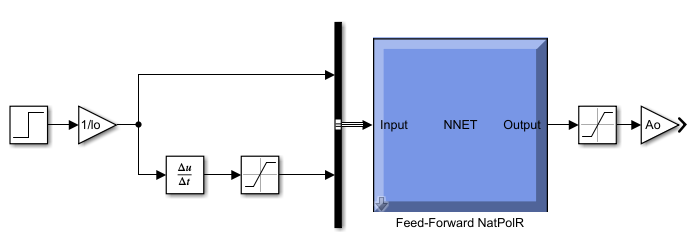
\includegraphics[width=\textwidth]{ANNStepTest.png}
    \caption{ Simulink implementation of the ANN model. The ANN model takes the strain and strain rate as inputs, and delivers the stress response of the material in MPa as output. The gain blocks ensure that the units are congruent. }
    \label{fig:ANNStepTest}
\end{figure}

The stress response of the ANN model for a Step input is in accordance to the values reported in \Cref{fig:NatRoff}. The ANN model outputs a negative stress values when a zero strain and zero strain rate are given as inputs. The latter could be a consequence of not providing enough data to the ANN during training for the zero input scenario. Nonetheless, a negative stress output is not realistic since the soft material will only have reaction forces under uni-axial extension. Therefore, a saturation block is used to prevent the latter. Similarly, the strain rate input is saturated to avoid presenting the ANN model with large values and negative values, and also to keep the strain range variation inside the ranges of values used during training, from 50 mm/min to 500 mm/min.

The stress response of the ANN model showed an unstable behaviour for a sine wave input signal. In this case, the ANN model performance was affected by both the frequency and the amplitude of the signal, as illustrated in \Cref{fig:ANNSineTesta,fig:ANNSineTestb,fig:ANNSineTestc}. This could be related to the fact that the strain rate in this scenario is changing over time, whereas the strain rate used for training was fixed between three different values. This however, does not indicate that the ANN model is not able to generalize well with other constant strain rates, as the one present in a tensile strength test. Nonetheless, this shows an unexpected limitation of the developed ANN model when being implemented as part of a control system. In contrast, the stress response of the ANN model was stable when using a constant strain rate as illustrated in \Cref{fig:ANNSineTestd}.

\begin{figure}[htb!]
	\centering
    \begin{subfigure}[b]{0.49\textwidth}
        \centering
        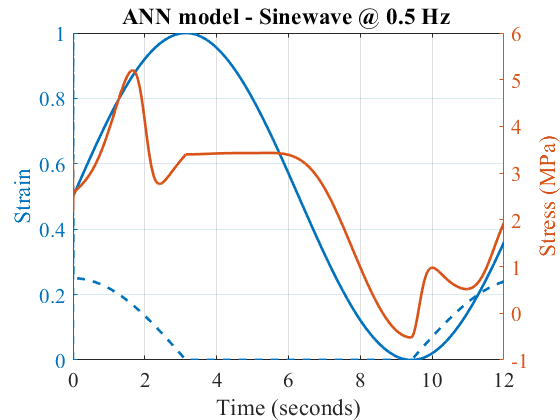
\includegraphics[width=\textwidth]{ANNSineResponse_HalfHz.png}
        \caption{}
        \label{fig:ANNSineTesta}
    \end{subfigure}
    \begin{subfigure}[b]{0.49\textwidth}
        \centering
        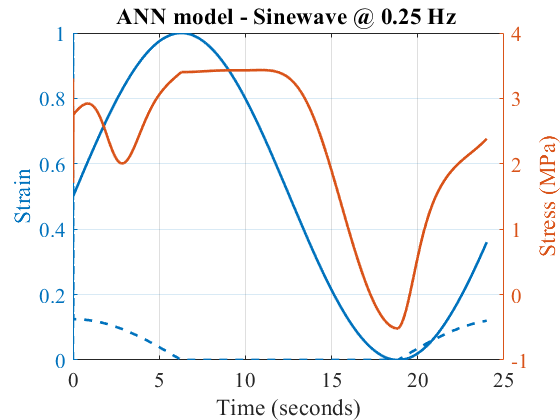
\includegraphics[width=\textwidth]{ANNSineResponse_QuarterHz.png}
        \caption{}
        \label{fig:ANNSineTestb}
    \end{subfigure}
    \begin{subfigure}[b]{0.49\textwidth}
        \centering
        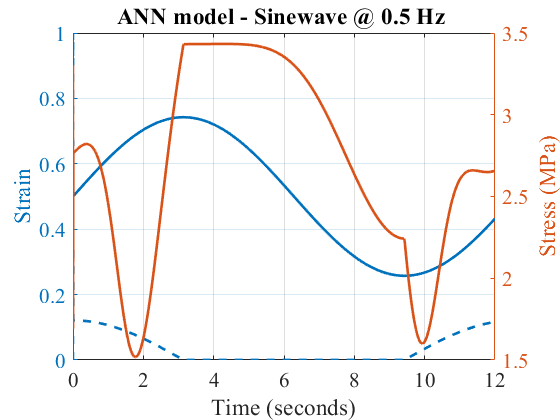
\includegraphics[width=\textwidth]{ANNSineResponse_HalfHz_HalfA.png}
        \caption{}
        \label{fig:ANNSineTestc}
    \end{subfigure}
    \begin{subfigure}[b]{0.49\textwidth}
        \centering
        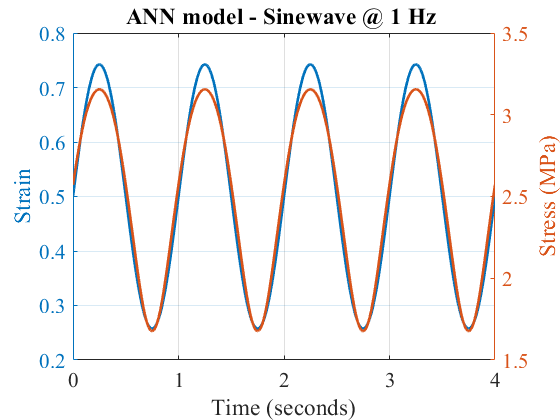
\includegraphics[width=\textwidth]{ANNSineResponse_1Hz_FixSR.png}
        \caption{}
        \label{fig:ANNSineTestd}
    \end{subfigure}
    \caption{ANN model stress response to a sine wave strain input. The solid and dotted blue line are the strain and strain rate, respectively. The ANN model response is affected by both the frequency (a), (b), and the amplitude (c) of the input signal. Also, the ANN model is only stable when the strain rate presented to it is constant, as in (d)}
    \label{fig:ANNSineTest}
\end{figure}

The latter test provided useful information about the behaviour of the ANN model under different input signals in real-time. An important limitation was found, which is the erratic prediction of the ANN model when the strain rate varies over time. The lack of zero input cases in the training data could be the reason for this and must be addressed to develop a robust ANN model. Nonetheless, a recent publication from last year \cite{xu2019artificial} , described a successful implementation of ANN models for the prediction of the elastic modulus of the material under different strain rates. The studied material was a graphene reinforced composite, and was characterized using a dynamic mechanical analysis over a range of frequencies and temperatures. These ranges of values are the input of the ANN model which in fact, does not directly predict the stress response of the material but it predicts the storage modulus of the material, a parameter known to describe the viscoelastic properties of materials. With this parameter, the stress response of the material can be extracted using known mathematical equations. The fact that ongoing research is being done on ANN model for the prediction of the velocity-dependent stress response of the materials highlights the relevance and feasibility of the research presented in here.

\section{Preliminary Design Concept of a Series-viscoelastic Actuator}

Series and parallel elastic actuators have been implemented in human assistance applications to achieve a muscle-like performance and increase the assistance capability of the robotic wearable devices. Traditionally, the mechanical element used to provide elasticity in actuators is a metallic spring. However, the idea of replacing the metallic spring with a soft material, such as rubber, is being researched now. The works performed by D. Rollinson has proved this idea to be beneficial for series elastic actuators (SEA) by developing a rotational spring based on natural rubber \cite{rollinson2013design,rollinson2014design}. In fact, the latter research gave birth to HEBI Robotics and to the first SEA implementing a soft material as the elastic element \cite{HEBI2019}. In addition to, other SEA concepts implementing rubber \cite{austin2015control}, dielectric elastomer \cite{bolivar2016towards} and polyurethane \cite{martins2015polyurethane} are being researched.

The benefits of series and parallel elasticity have been proved in many works both with rigid and soft materials as the elastic element. However, there is only one actuator concept documented in the literature which implements both series and parallel elasticity in the same actuator, creating a series-parallel elastic actuator (SPEA) \cite{mathijssen2014variable}. This actuator implements rigid springs and is based on the variable recruitment process observed in human muscles, which means that depending on the required torque and displacement, more springs will be engaged.

As previously mentioned, an assistive commonly aims to reduce the workload of the wearer by 50\%. In this research, particular focus was put into the knee joint due to its contributions in the activities of daily living. In line with this, the required peak torque and angular speed range for the knee joint during normal walking was found to be 29 Nm and $\pm$50 rpm respectively \cite{dos2014impedance,winter2009biomechanics}. Therefore, the peak torque aimed to be delivered to achieve a 50\% assistance is 18 Nm. The previous parameters will be used as guidelines when selecting the electric motor/gearbox combination to be used in the simulation. Another important working range is the one from the soft material. The latter is indicated by the elastic region of the material, which was approximated using the offset yield strength in \Cref{sec:CharacterizationProcess}. In summary, the parameters aimed to be use in a future experimental validation are presented in \Cref{tbl:simParameters}.

\begin{table}[hbt!]
    \centering
    \caption{Simulation parameters}
    \begin{tabular}{ll}
    \toprule
    Soft Material       & Natural Rubber with Polyester (NatPolR)\\
    Working Range       & Up to 0.5 strain ( 16.5 mm)\\
    Strip Width        & 20 mm\\
    Strip length       & 33 mm\\
    $A_o$               & 9 $mm^2$\\
    No. of strips      & 8\\ 
    Torque reference    & Knee joint motion capture data \\
    Position reference  & Knee joint motion capture data \\
    \midrule
    Electric motor      & Maxon RE53-323891 \cite{Maxon2019motor}\\
    Nominal Voltage     & 24 V\\
    $L_a$               & 0.191 mH\\
    $R_a$               & 0.583 $\Omega$\\
    $K_a$               & 29.2 mNm/A\\
    $K_b$               & 0.029 V/(rad/s)\\
    $J_m$               & 79.2 g/$cm^2$\\
    \midrule
    Gearbox             & Maxon GP 42 C-203124 \cite{Maxon2019gearhead}\\
    $n$                 & 1/81\\
    \end{tabular}
    \label{tbl:simParameters}
\end{table}

As part of the preliminary design of the series-viscoelastic actuator, and in line with using a bundle of soft materials to mach the human tendon mechanical properties, a clamping device was designed in SolidWorks (\Cref{fig:ClampWhole}). The width proposed in the matching factor process of previous sections was based on the dimensions of this clamping device. The idea behind this design is to stack several pieces of the same material on top of each other and then clamp them together to create a bundle of soft materials. This design is similar to the one used in the literature when dealing with rubber materials and cable-driven actuators \cite{austin2015control}.

\begin{figure}[htb!]
	\centering
    \begin{subfigure}[b]{0.49\textwidth}
        \centering
        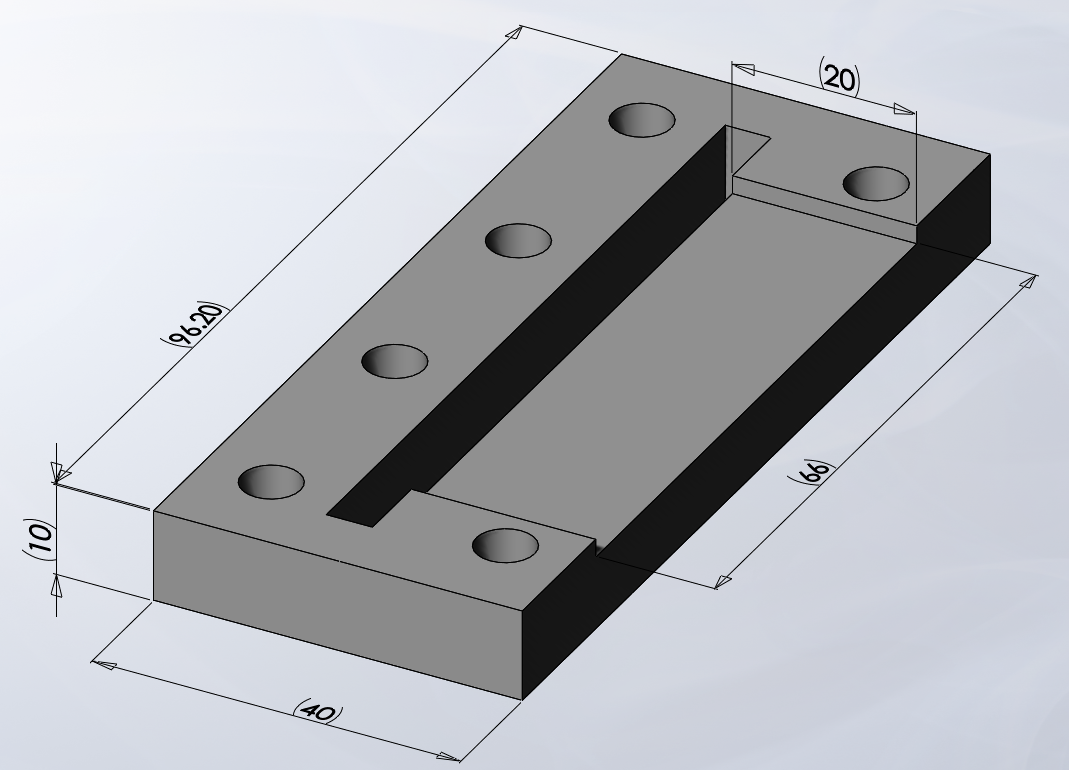
\includegraphics[width=\textwidth]{ClampBase.PNG}
        \caption{}
        \label{fig:ClampBase}
    \end{subfigure}
    \begin{subfigure}[b]{0.49\textwidth}
        \centering
        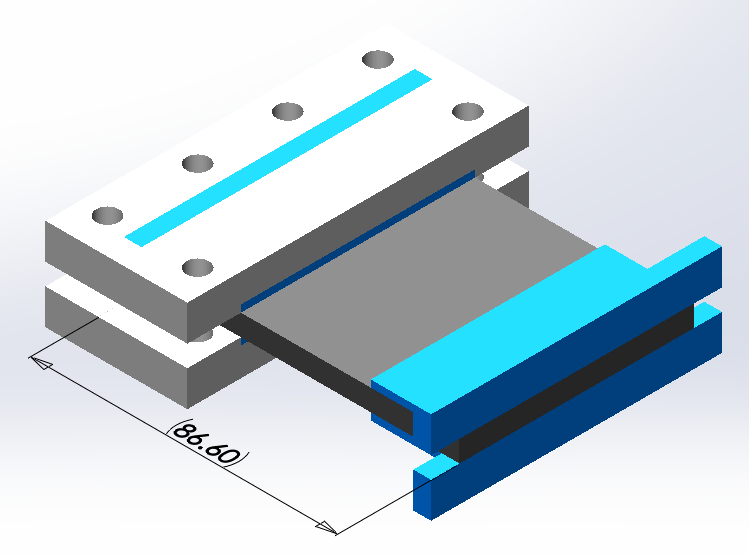
\includegraphics[width=\textwidth]{ClampedElement.PNG}
        \caption{}
        \label{fig:ClampElement}
    \end{subfigure}
    \caption{(a) Bottom part of the detachable clamping device designed, (b) Example of final assembly, the soft material is coloured in black, and the T-shape attachment in blue. The latter attachment function as ``plug and play", which allows the quick testing of different bundles of soft materials. Units in millimeters.}
    \label{fig:ClampWhole}
\end{figure}

The clamp mechanism of \Cref{fig:ClampWhole} was designed to be detachable. This is achieved by having a T-shape element which can be glued to a bundle of materials strips. Each soft material strip must also be glued to each other to allow for even deformation of the whole bundle. The T-shape attachment fits inside the clamp base (\Cref{fig:ClampBase}) and also in the clamp top element. Once in place, the clamp mechanism can be secured with bolts going through the holes added to the clamp base and top parts. This is illustrated in \Cref{fig:ClampElement}. As previously mentioned, this design was inspired in the one used in \cite{austin2015control}, with the addition of designing it as detachable clamping mechanism to allow the test of different soft materials bundles, when being used as part of a test bench. This clamping mechanism was not manufactured.

Finally, an experimental protocol was designed and documented as well (\Cref{appendixB}). The tests proposed in there aim to investigate the concept of variable recruitment in soft cable-driven actuators, i.e. series-viscoelastic actuators. In addition to this, the concept of co-contraction is also aimed to be investigated.

\section{Summary}

In this chapter, the preliminary design concept of a series-viscoelastic actuators was presented. As the very first step in the design process and in line with the aim of mimicking the human muscle skeletal system, the comparison of the human tendon mechanical properties against the soft materials was made. In addition to this, the validation of the ANN model performance under real-time conditions was performed. The results were unexpected due to the erratic stress response prediction of the ANN model. The latter is directly related with the fact that only up to three different strain rates were included in the training set. Moreover, the stress response of the ANN model is also affected by the selection of frequency and amplitude of the strain input. Nonetheless, the ANN model was able to follow a sine wave strain input when having a constant strain rate in its input. The latter limitation must be addressed in future works to develop a robust ANN model.

Finally, the work related to the design process of the series-viscoelastic actuator was presented, which included: the selection of actuator technologies, selection of the best soft material to match the human tendon properties, design of a clamping device to hold a bundle of stacked soft material pieces, and the designed experimental protocol which can be found in the \Cref{appendixB}.